\documentclass{protokol}
\leftheader{Michelsonův interferometr}
\centerheader{Praktikum III}
\rightheader{Tomáš Derner}

\begin{document}

  \section*{Úkol}

    \begin{enumerate}
      \item Změřte divergenci laserového svazku. Průměry svazku změřte na milimetrovém papíru i měřičem profilu svazků a obě metody porovnejte.
      \item Sestavte Galileův teleskop. Změřte, kolikrát rozšiřuje průměr svazku, a výsledek porovnejte s výpočtem rozšíření ze známých ohniskových délek čoček.
      \item Sestavte Michelsonův interferometr. Vysvětlete princip vzniku interferenčních proužků.
      \item Pozorujte, popište a vysvětlete změny v interferenčním obrazci při:
      \begin{enumerate}
        \item naklánění zrcadla Z4,
        \item posunu zrcadla Z3 mikrometrickým šroubem,
        \item vkládání skla do svazku ve čtyřech polohách kolem děliče svazku a
        \item ohřátí vzduchu v různých místech průchodu svazku.
      \end{enumerate}
    \end{enumerate}

  \section*{Teorie}

    Cílem tohoto praktika bylo sestavit funkční Michelsonův interferometr pomocí základních komponent podle obrázku \ref{fig:diagram}. Použit byl helium-neonový laser, zrcadla $Z_1$ - $Z_4$, rozptylná čočka $C_1$, spojná čočka $C_2$, dělič svazku $DS$ a dvě stínítka $S_1$ a $S_2$.
    
    \begin{figure}[H]
      \centering
      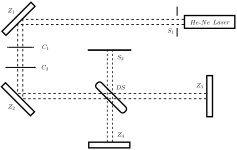
\includegraphics[width=\textwidth]{diagram}
      \caption{Diagram sestavení Michelsonova interferometru}
      \label{fig:diagram}
    \end{figure}
    
    Divergencí svazku je obvykle myšlen zlomek
    \begin{equation}
      d_o = \frac{D_2-D_1}{s},
    \end{equation}
    kde $D_1$ je průměr svazku v místě výstupního otvoru laseru a $D_2$ průměr svazku ve vzdálenosti $s$. Protože však není jistéjaký průběh má tvar svazku v těsné blízkosti výstupního otvoru laseru, bereme zde divergenci jako 
    \begin{equation} \label{eq:divergence}
      d = \frac{D_b - D_a}{b-a},
    \end{equation}
    kde $D_a$ a $D_b$ jsou průměry svazku ve vzdálenosti $a$ resp. $b$ od výstupního otvoru laseru ($a < b$).
    
  \section*{Výsledky}

    \subsection*{Úkol 1}
      Pro určení divergence svazku metodou projekce na milimetrový papír jsme změřili průměr svazku ve vzdálenosti $a = \SI{0.78 \pm 0.01}  {m}$
      $$ D_a = \SI{2.5 \pm 0.7}{mm} $$
      a ve vzdálenosti $b = \SI{2.49 \pm 0.1}{m}$
      $$ D_b = \SI{6 \pm 1}{mm}. $$

      Dosazením těchto hodnot do vztahu \eqref{eq:divergence} získáme divergenci svazku
      $$ d_\text{I} = \num{0.002 \pm 0.0007}. $$

      Pomocí měřiče profilu svazku byly změřeny průměry svazku v osách $X$ a $Y$ v oblasti $\frac{1}{e^2}$ násobku amplitudy ve vzdálenosti $a = \SI{0.77 \pm 0.01}{m}$ od výstupního otvoru laseru
      $$ D_{a, X} = \SI{1090 \pm 30}{\micro\metre}, $$
      $$ D_{a, Y} = \SI{1120 \pm 30}{\micro\metre} $$
      a ve vzdálenosti $\SI{2.49 \pm 0.1}{m}$
      $$ D_{b, X} = \SI{3015 \pm 30}{\micro\metre}, $$
      $$ D_{b, Y} = \SI{2940 \pm 30}{\micro\metre}. $$
       
      Jako průměr laserového svazku uvažujeme aritmetický průměr hodnot v obou souřadnicích
      $$ D_a = \SI{1105 \pm 30}{\micro\metre}, $$
      $$ D_b = \SI{2978 \pm 30}{\micro\metre}. $$

      Dosazením do vztahu \eqref{eq:divergence} získáme divergenci svazku
      $$ d_\text{II} = \num{0.00109 \pm 0.00007}. $$

    \subsection*{Úkol 2}

      Jako první byly na optickou desku umístěny zrcadla $Z_1$ - $Z_3$ seřízená tak, aby se laserový svazek promítal zpět na stínítko $S_1$ co nejblíže k výstupnímu otvoru laseru. Následně byla mezi zrcadla $Z_1$ a $Z_2$ vložena rozptylná čočka $C_1$ s ohniskovou vzdáleností $f_1 = \SI{-25}{mm}$ a spojná čočka s ohniskovou vzdáleností $f_2 = \SI{200}{mm}$ tak, aby společně sdílely ohnisko. Průměr svazku vystupujícího z této soustavy je 
      $$ D_s = \SI{12 \pm 1}{mm}. $$

    \subsection*{Úkol 3}

      Dále byl na optické desce postaven Michelsonův interferometr podle diagramu \ref{fig:diagram}. Jeho princip spočívá v interferenci dvou svazků rozdělených děličem svazku $DS$ a odražených zrcadly $Z_3$ a $Z_4$. Ke střídání světlých a tmavých proužků dochází kvůli mírnému natočení zrcadla $Z_4$ od směru kolmého dopadu svazku, délka ramene se tedy mírně liší v závislosti na místě odrazu od $Z_4$ a tedy i na místě dopadu na stínítko.

    \subsection*{Úkol 4}

      Nakláněním zrcadla $Z_4$ je možné měnit hustotu interferenčních proužků a jejich směr. Z vysvětlení výše plyne, že čím větší je náklon zrcadla od kolmého směru dopadajícího svazku, tím více uvidíme interferenčních proužků. Zároveň platí, že natáčením podle svislé osy nastavujeme počet svislých proužků, podle svislé horizontální nastavujeme počet horizontálních proužků (pakliže je druhé natočení nulové). Odpovídají-li si obě natočení, proužky jsou diagonální. Lze také pozorovat efekt přetočení proužků přetočíme-li zrcátko z jedné strany na druhou.

      Při posunu zrcadla $Z_3$ dopředu či dozadu se posouvají interferenční proužky.

      Vložením skla mezi dělič svazku a zrcadlo $Z_3$ či $Z_4$ dojde k deformaci proužků. Plochy skla nejsou totiž dokonale rovnoběžné a tvoří klín, což tedy vlivem vyššího indexu lomu v různých místech prodlužuje optickou dráhu více než jinde. Vložení skla před dělič svazku má minimální efekt.

      Zahřátím vzduchu mezi děličem svazku a zrcadlem $Z_3$ či $Z_4$ dojde k chaotickému pohybu interferenčních proužků, protože teplý vzduch má odlišný index lomu. Určitý efekt je pozorovatelný i při ohřátí vzduchu před děličem svazku.

  \section*{Diskuse}

    Divergence svazku měřená milimetrovým papírem se liší dvojnásobně od hodnoty měřené digitálně. První z těchto měření je však zatíženo značnou chybou, výrazným důvodem tohoto rozporu může být také skutečnost, že na milimetrovém papíru byla šířka svazku měřená od jedné strany světelné stopy ke druhé nehledě na intenzitu světla zatímco digitálně byl měřen průměr svazku s hraniční intenzitou $\frac{1}{e^2}$ amplitudy.

  \section*{Závěr}

    Byla naměřena divergence svazku pomocí milimetrového papíru
    $$ d_\text{I} = \num{0.002 \pm 0.0007} $$
    a pomocí měřiče profilu svazku 
    $$ d_\text{II} = \num{0.00109 \pm 0.00007}. $$

    Byl sestaven Galileův dalekohled, který rozšířil svazek na průměr
    $$ D_s = \SI{12 \pm 1}{mm}. $$

    Byl sestaven Michelsonův interferometr, byla vysvětlena jeho funkce a změny interferenčního obrazce při různých manipulacích.

  \begin{thebibliography}{}
 
    \bibitem{pokyny}
    Pokyny k měření ``Stavba Michelsonova interferometru a ověření jeho funkce'', dostupné z\\ \url{http://physics.mff.cuni.cz/vyuka/zfp/_media/zadani/pokyny/mereni_320.pdf}, 18.\,4.\,2018
   
  \end{thebibliography}

\end{document} 